\chapter{Circuito Limitador Básico}
El circuito limitador básico está compuesto por una resistencia en serie y dos Diodos Zener enfrentados, configurados como se observa en la figura \ref{fig:limitador_basico}.

\begin{figure}[ht]
    \begin{center}
        \begin{circuitikz}[american voltages]
    \draw
    (0,0) node[ocirc](Vi-){}
    (0,4) node[ocirc](Vi+){}
    (5,0) node[ocirc](Vo-){}
    (5,4) node[ocirc](Vo+){}
    (Vi+) to[R=$R_s$,-*] ++(3,0)
    to[zzD*, l=$D_{z1}$] ++(0,-2)
    (Vi-) to[short, -*] ++(3,0)
    to[zzD*, l=$D_{z2}$] ++(0,+2)
    (Vo+) -- ++(-2,0)
    (Vo-) -- ++(-2,0)
    (Vi+) to[open, v=$V_i$] (Vi-)
    (Vo+) to[open, v=$V_o$] (Vo-)
    ;
\end{circuitikz}
\caption{Circuito Limitador Básico}
        \label{fig:limitador_basico}
    \end{center}
\end{figure}

\section{Funcionamiento} \label{funcionamiento}
Para analizar la operación del circuito se puede pensar en los siguientes casos:

\begin{enumerate}
    \item $|V_i| \leq V_F$
    \item $V_F < |V_i| \leq V_z + V_F$
    \item $V_z + V_F < |V_i|$ 
\end{enumerate}

Dado que los diodos están enfrentados, el comportamiento de este circuito será el mismo tanto para tensiones negativas como positivas.

En el primer caso, como la tensión no es suficiente ni siquiera para polarizar $D_{z1}$, no hay flujo de corriente, por lo tanto la tensión a la salida es $V_o = V_i$. En el segundo caso, la tensión es suficiente para polarizar en directa $D_{z1}$, y $D_{z2}$ se polariza en inversa, pero no alcanza $V_z$ para activarse el modo Zener. Se puede considerar entonces que, dado que la corriente en inversa es despreciable, no hay flujo de corriente y la tensión de salida copia a la de entrada.

En el tercer caso, la tensión de entrada es suficiente para polarizar $D_{z1}$ en directa y en $D_{z2}$ superar la tensión de Zener. Cuando el circuito está operando en esta región, se lo puede interpretar como se observa en la figura \ref{fig:limitador_activado}. A este punto, la salida del circuito estará dada por la expresión \eqref{eqn:transferencia}.

\begin{equation}
    \frac{V_o - (V_F + V_z)}{V_i - (V_F + V_z)}=\frac{r_z}{R_s + r_z}
    \label{eqn:transferencia}
\end{equation}

\begin{figure}[ht]
    \begin{center}
        \begin{circuitikz}[american voltages]
    \draw
    (0,0) node[ocirc](Vi-){}
    (0,4) node[ocirc](Vi+){}
    (5,0) node[ocirc](Vo-){}
    (5,4) node[ocirc](Vo+){}
    (Vi+) to[R=$R_s$,-*] ++(3,0)
    to[battery1, l=$V_F$] ++(0,-2)
    (Vi-) to[short, -*] ++(3,0)
    to [battery1, invert, l=$V_z$] ++(0,1) to[R, resistors/scale=0.5, l=$r_z$] ++(0,1) 
    (Vo+) -- ++(-2,0)
    (Vo-) -- ++(-2,0)
    (Vi+) to[open, v=$V_i$] (Vi-)
    (Vo+) to[open, v=$V_o$] (Vo-)
    ;
\end{circuitikz}
\caption{Circuito Limitador Activado}
        \label{fig:limitador_activado}
    \end{center}
\end{figure}

\section{Selección de Componentes}

Se escogió trabajar con el diodo BZX55C3V6, el cual tiene una tensión típica de zener de $V_z = 3.6 \si{\volt}$ y una potencia máxima $P_{max} = 0.5 \si{\watt}$. A partir de estos datos se obtuvo que la corriente máxima que puede circular por el diodo.

\begin{equation}
    I_{max}=\frac{P_{max}}{V_z}
\end{equation}

Luego, la $R_s$ que se debe utilizar estará dada por:

\begin{equation}
    R_{min}=\frac{V_i-(V_z+V_F)}{I_{max}}-r_z
\end{equation}

La mayor $R_{min}$ se obtuvo no tomando la caída de tensión en directa y la resistencia del diodo zener.

\begin{equation}
    R_{min}=\frac{V_i-V_z}{I_{max}}
\end{equation}

Finalmente los componentes y datos obtenidos fueron los siguientes:

\begin{table}[ht]
    \begin{center}
        \begin{tabular}{|l|r|r|r|r|}
            \hline
            Diodo & $V_z$ & $P_{max}$ & $I_{max}$ & $R_{min}$ \\
            \hline
            BZX55C3V6 & $3.6 \si{\volt}$ & $0.5 \si{\watt}$ & $0.139 \si{\ampere}$ & $46.08 \si{\ohm}$ \\
            \hline
        \end{tabular}
        \caption{Restricciones de los componentes del circuito}
        \label{tabla_limitador}
    \end{center}
\end{table}

\begin{table}[ht]
    \begin{center}
        \begin{tabular}{|l|r|r|r|r|}
            \hline
            Diodo & $V_z$ & $r_{\text{z max}}$ & $R_s$ & $V_{\text{F max}}$\\
            \hline
            BZX55C3V6 & $3.6 \si{\volt}$ & $80 \si{\ohm}$ & $100 \si{\ohm}$ & $1.5 \si{\volt}$ \\
            \hline
        \end{tabular}
        \caption{Componentes Utilizados y Características}
    \end{center}
\end{table}

La resistencia fue elegida de modo que el incremento en la caída de tensión, una vez que 
los diodos estén en modo zener, sea bajo. Para las mediciones se utilizó una 
resistencia de $100\Omega$.

\section{Resultados}

\subsection{Teóricos}
Teniendo en cuenta los valores de los componentes, y conociendo el comportamiento ideal 
del circuito, se sabe que cuando $|V_i|< V_F+V_z$ la tensión de salida sigue a la entrada.

Fuera de esta región, la recta tendrá una pendiente de $\frac{r_z}{R_s+r_z}$.
\subsection{Simulación}
Se utilizó la siguiente configuración para simular el comportamiento del circuito


\begin{figure}[H]
    \begin{center}
        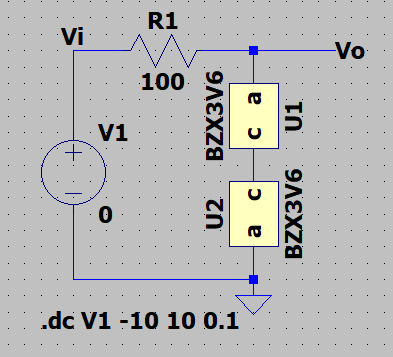
\includegraphics[width=9cm]{limitador/limitador_spice.png}
        \caption{Configuración del circuito en LTSpice XVII}
    \end{center}
\end{figure}

\subsection{Prácticos}
<<Mostrar y explicar cómo medimos las cosas>>

\begin{figure}[H]
    \begin{center}
        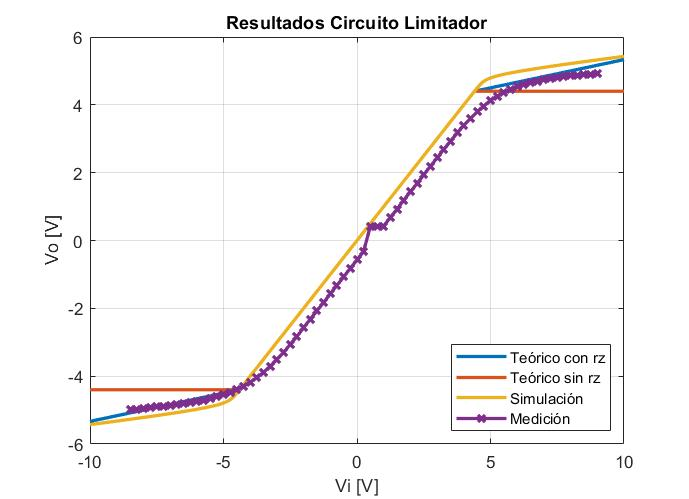
\includegraphics[width=12.7cm]{limitador/figures.jpg}
        \caption{Resultados de las mediciones}
    \end{center}
\end{figure}

\subsection{Ganancia de tensión}
En esta sección se realizará el análisis de la ganancia de tensión del circuito 
presentado en [\ref{fig:limitador_basico}]. \par 
Se considerarán dos casos, con y sin $R_z$, cuyo valor teórico fue previamente presentado 
en [\ref{tabla_limitador}].
Se estudiará la ganancia de tensión sobre tres zonas bien diferenciadas como ya se 
presento en \ref{funcionamiento}. Los gráficos obtenidos se presentan a continuación.






\subsection{Implementación}
Para medir el circuito limitador se implementó el mismo en la protoboard del 
\textit{Electronic Explorer} como se puede ver en la imagen [\ref{implementacion_limitador}].
Se utilizaron tres puntas para medir la tensión en la entrada, en la salida y sobre cada 
diodo. \par 
Se utilizaron scripts para realizar un \textit{DC Sweep} sobre el circuito en el rango 
$\pm 9V$, limitiación impuesta por el equipo.


\begin{figure}[H]
    \begin{center}
        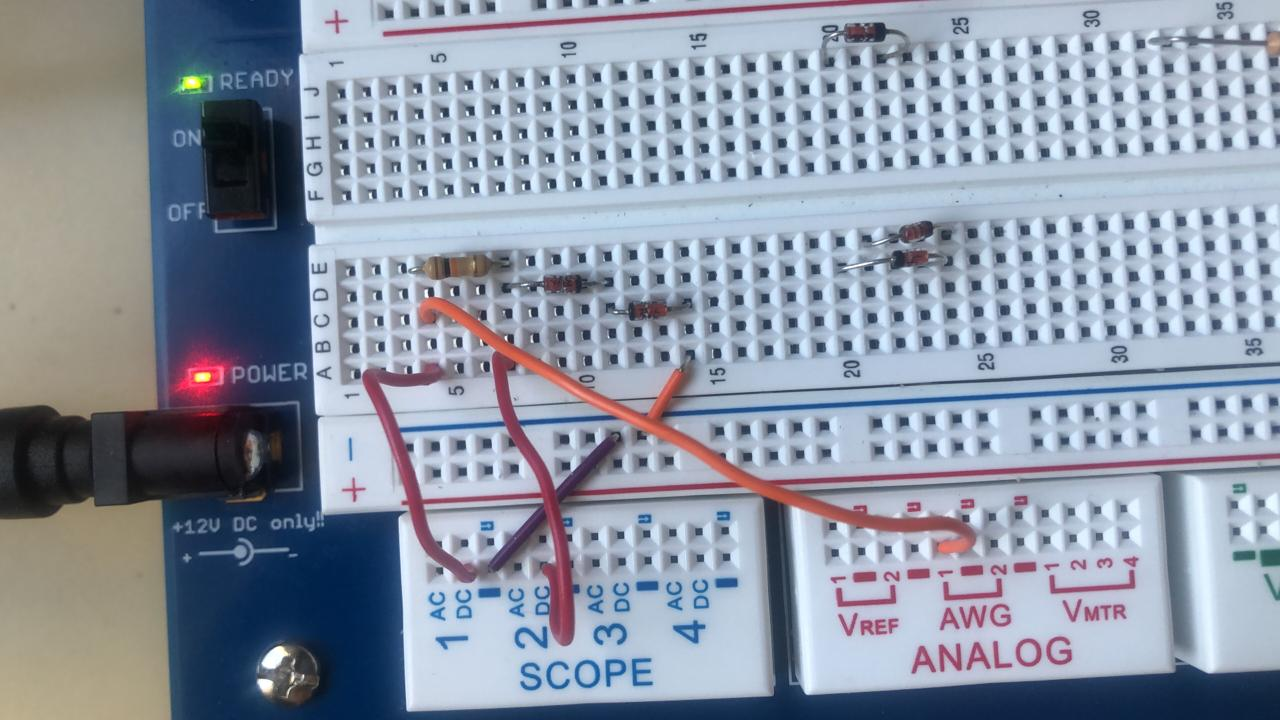
\includegraphics[width=0.7\textwidth]{limitador/Imagenes/foto_medicion_limitador.jpeg}
        \caption{Implementación del circuito}
        \label{implementacion_limitador}
    \end{center}
\end{figure}
